%=======================================================================
% SM 4/2017
% Master's thesis Report IISER Thiruvananthapuram
% Investigations of SpinTaylorF2
%=======================================================================

\chapter{Bounds on $\chi_1$}

\subsection{Bounds on $\chi_1$ and $\kappa$}

We have seen that if either the $m=2$ or the $m=0$ mode dominates, i.e., the
system is in region~(b) or (a), we can assert whether the binary is either
non-precessing or strongly precessing. If we assume the spin harmonics to be
orthogonal\footnote{The simulations show that for the regions of interest,
where both $m=2$ and $m=0$ modes are relevant, the maximum values of overlap
between $\tilde h_2(f)$ and $\tilde h_0(f)$ is less than $0.15$.}, we can
express the SNR of a particular spin harmonic $m$ as
\begin{equation}
\text{SNR}_{m} = H_{m} (\theta_{J}, \psi'_J) (\hslash_{m}(\eta,
\kappa,\chi_1)\,|\,\hslash_{m}(\eta, \kappa,\chi_1))^{1/2},
\label{EQ:SNR_split}
\end{equation}
where $\text{SNR}_{m}$ corresponds to the SNR of spin harmonic $m$, $H_{m}$ is
the waveform amplitude that depends only on the orientation of the source and
$\hslash_{m}$ depends on the intrinsic parameters of the source $(\eta,
\kappa,\chi_1)$ though $\alpha(f), \beta(f), \zeta(f)$ and $\Psi(f)$. Using
Eq.~(\ref{EQ:SNR_split}) we can define a function $\Sigma(\eta, \chi_1,
\kappa)$ expressed in terms of the SNR ratio of the $m=2$ and $m=0$ spin
harmonics and their amplitude ratio $H_{0}/H_{2}$ as
1
\begin{equation}
\Sigma(\eta, \chi_1, \kappa):=\frac{(\hslash_{2}\,|\,\hslash_{2})^{1/2}}{(\hslash_{0}\,|\,\hslash_{0})^{1/2}} =
\left(\frac{\text{SNR}_{2}}{\text{SNR}_{0}}\right)_{(\eta,\,\chi_1,
\,\kappa)} \times \left(\frac{H_{0}}{H_{2}}\right).
\label{EQ:Sigma}
\end{equation}

We discuss the implications of Eq.~(\ref{EQ:Sigma}). If we measure the SNR
ratio of the two spin harmonics, and fix the amplitude ratio $H_0/H_2$, it
restricts the range of parameters in the $(\eta,\,\chi_1,\,\kappa)$ parameter
space, which helps puts bounds on the possible values of $\kappa$ and $\chi_1$
for a given value of $\eta$. Below, we explore the bounds on these two
parameters ($\chi_1$ and $\kappa$) for the given value of $\eta$ and
$H_0/H_2$\footnote{We do not refer to corresponding values of $\theta_J$ and
$\psi_J$ for a given value of $|H_0/H_2|$ since the value of the function
$|H_0/H_2|$ is degenerate in $\theta_J$ and $\psi_J$.}, when
$\text{SNR}_2/\text{SNR}_0 \sim 1$, for simplicity. For our analysis, we have
considered the BH spin ($\chi_1$) to vary between $0.2$ and $0.8$.

\begin{figure}[!htbp] 
\centering
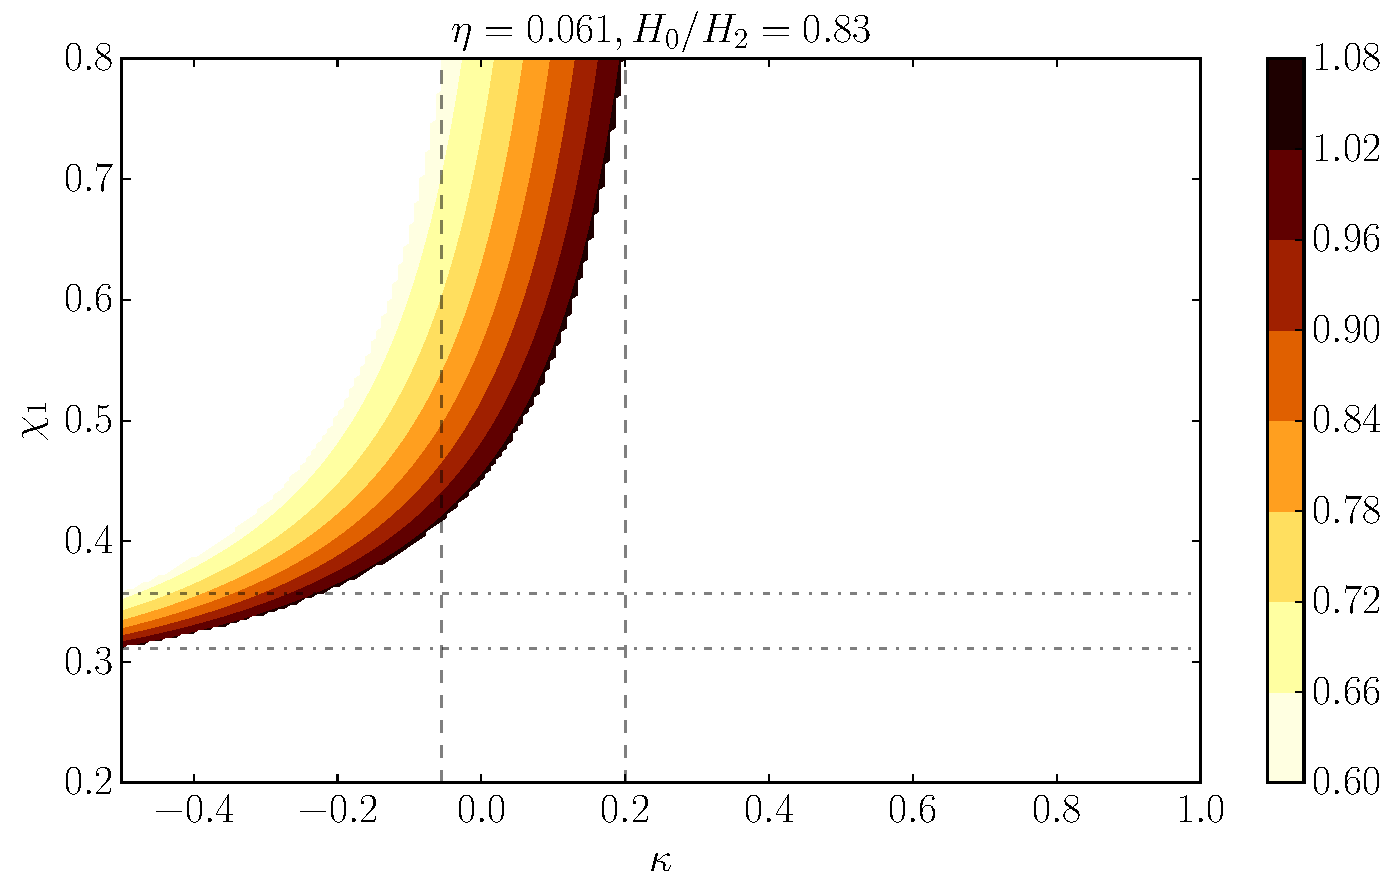
\includegraphics[width=0.55\linewidth]{images/SM_bounds.pdf} 
\caption{\small{Region of $(\chi, \kappa)$ parameter space for $\eta=0.06$,
$H_{0}/H_{2}=0.83$, and for $\text{SNR}_2/\text{SNR}_0$ restricted between
0.75 and 1.25.}}
\label{FIG:chi_kappa_region}
\end{figure}

In Fig.~\ref{FIG:chi_kappa_region}, we show the two dimensional region of
$(\chi_1$, $\kappa)$ parameter space for a fixed value of $\eta$ and
$H_0/H_2$, where the SNR ratio $(\text{SNR}_2/\text{SNR}_0)$ is allowed to
vary between between 0.75 and 1.25, to account for the uncertainty in the
measurements due to the presence of detector noise. The vertical dashed lines
correspond to the upper bound on the value of $\kappa$ and the spacing between
them represents the uncertainty in the bound, since we've considered a range
of SNR ratios close to 1. Similarly, the horizontal dotted lines and the
spacing between them corresponds to the lower bound on $\chi_{1}$ and it's
associated uncertainty respectively. The color bar represents the value of
$\Sigma(\eta, \chi_1,
\kappa)$ in these regions. The outer edge of the region corresponds to
$(\text{SNR}_2/\text{SNR}_0)=1.25$ and the inner edge corresponds  to the
regions where $(\text{SNR}_2/\text{SNR}_0)=0.75$. 

The variation in the value of $\Sigma(\eta, \chi_1, \kappa)$  is due to the
fact that $(\text{SNR}_2/\text{SNR}_0)$ is maximum for the non-precessing
case, i.e., $\chi_1=0$ and/ or $\kappa=1$ (since the $m=2$ spin harmonic
dominates in these regions) and is minimum for the highly precessing case
($\chi_1$ is close to 1 and $\kappa \leq 0$) where $m=0$  is the dominant
harmonic. Notice that the funnel shaped region in $(\chi,\,\kappa)$ plane
suggests that the SNR ratio varies much more rapidly along $\chi_1$ than along
$\kappa$, for negative values of $\kappa$. This implies, that for a highly
anti-aligned system we would be able to constrain the lower bound on $\chi_1$
more accurately than the upper bound on $\kappa$, which shows a larger
variation for the exact same parameter values.

We now investigate the variation of these bounds with $\eta$ (or equivalently
the BH mass, since the NS mass is fixed to $1.4M_\odot$) and the effective
orientation parameter $H_{0}/H_{2}$, which is a function of $\theta_J$ and
$\psi'_J$. We consider two values of $\eta$ that correspond to BH masses of
$17 M_\odot$ and $43.8 M_\odot$. Further, the ratio $H_{0}/H_{2}$ is
analytically bounded, and varies between $-1.5$ to $1.5$ over all values of
$\theta_J$ and $\psi'_J$. For our purposes we consider only the positive
values of $H_{0}/H_{2}$, since the bounds are symmetric about $H_0/H_2=0$.

\begin{figure}[!htbp] 
\centering
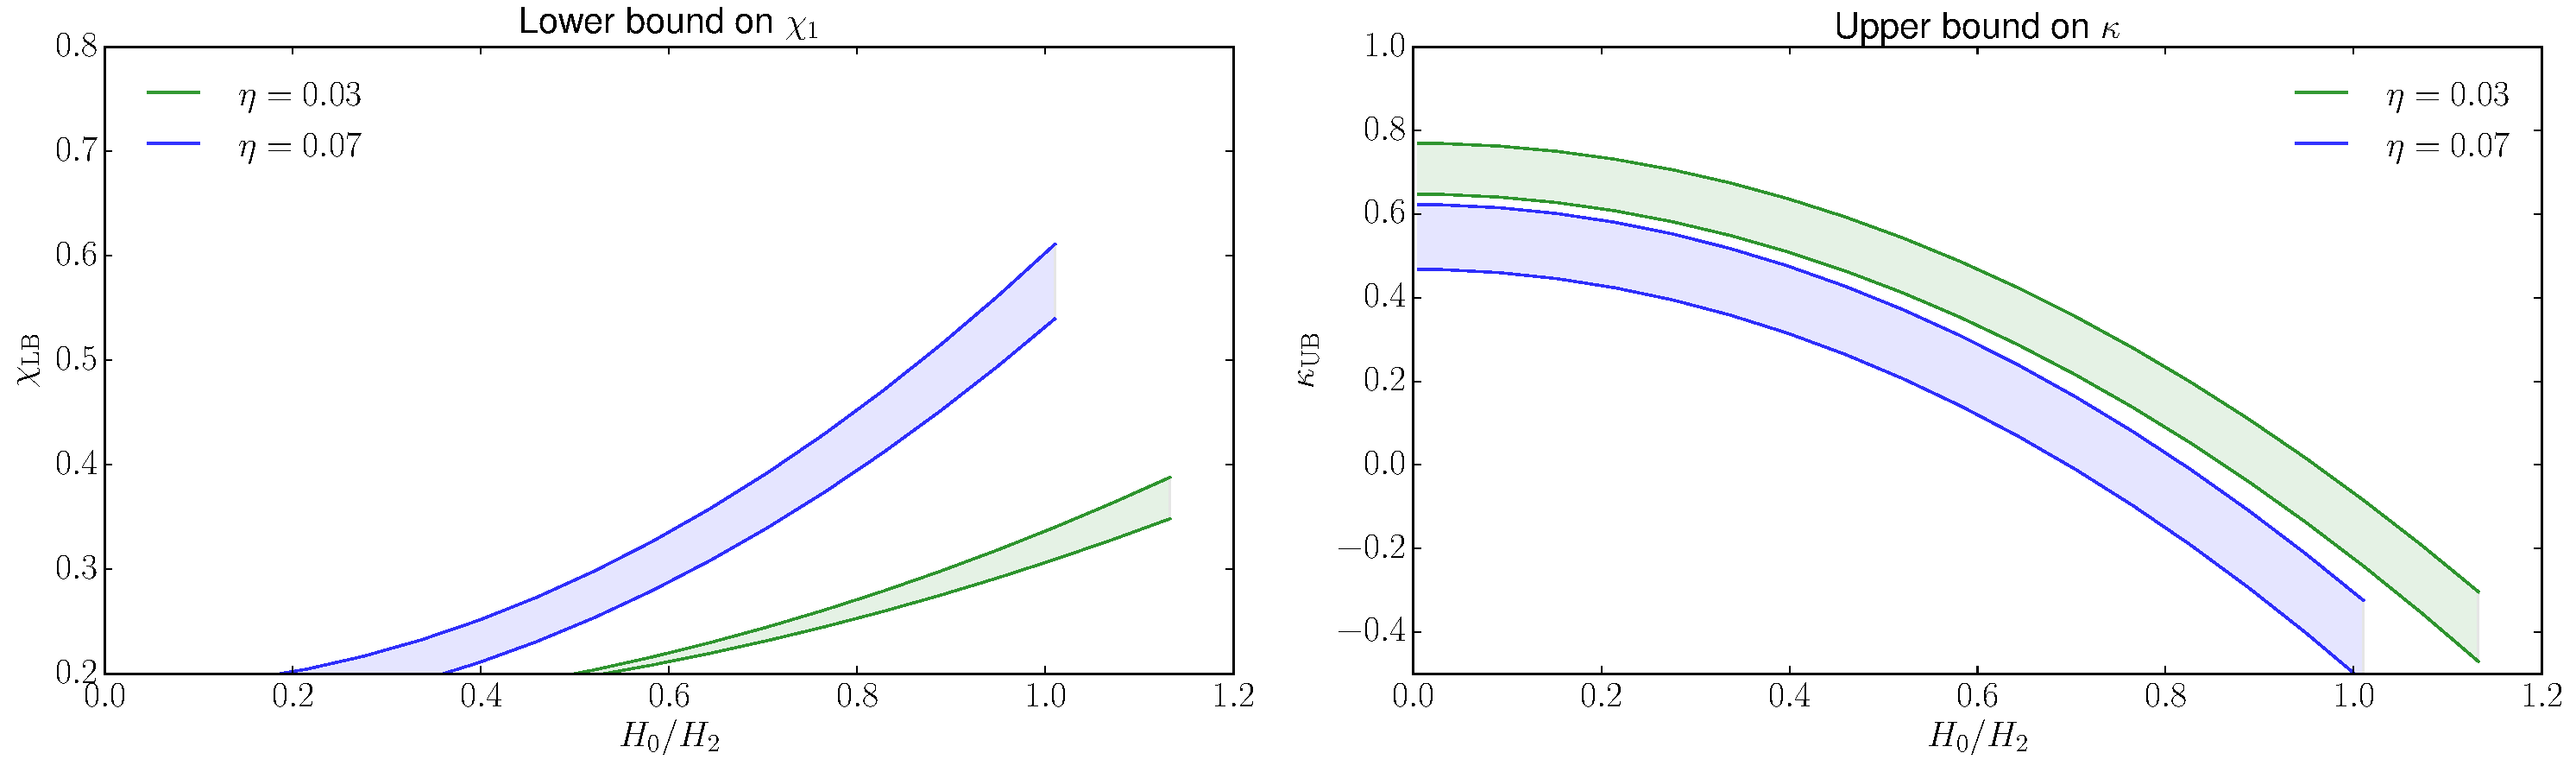
\includegraphics[width=\linewidth]{images/SM_chi_kappa_bounds.pdf}
\caption{\small{Variation of lower bound on $\chi_{1}$ (left) and upper bound on $\kappa$ (right)
for BH masses $17M_\odot$ and $43.8 M_\odot$. The shaded region bounded by the
solid lines correspond to the uncertainty in the value of the bound, for
particular value of $H_0/H_2$. }}
\label{FIG:chi_kappa_bounds}
\end{figure}

In Fig.~\ref{FIG:chi_kappa_bounds} we show the variation of these bounds over
$H_{0}/H_{2}$, for different values of $\eta$. As an example, consider the
bounds on $\chi_1$ and $\kappa$ for $\eta=0.07$, given $H_0/H_2=0.8$. 
For these values, from Fig.~(\ref{FIG:chi_kappa_bounds}) we can infer that the
lower bound on $\chi_1$  is $\sim 0.4$. This implies that, for the given set
of parameters, $\chi_1$ can only take values \textit{above} $0.4$, up to $1$,
if we require $\text{SNR}_2/\text{SNR}_0 \sim 1$. Similarly, for $\kappa$, we
observe that the upper bound on $\kappa$ is $\sim 0.2$, which suggests that
$\kappa$ can take values no higher than $\sim 0.2$, which translates into the
fact that highly aligned systems do not show orbital precession, and therefore
cannot give $\text{SNR}_2/\text{SNR}_0 \sim 1$. In both cases, however,
there's an uncertainty in these values, that corresponds to the width of the
shaded region at $H_0/H_2=0.8$.

We show that the bounds improve (i.e.,~the values of the parameters are better
constrained, in terms of the range over which they are allowed to vary) as
(i)~the value of $\eta$ increases or as the BH mass decreases and (ii)~for
higher values of $H_{0}/H_{2}$. The uncertainty in the value of the bounds,
however, follows the opposite trend---it increases with increasing value of
$\eta$ (clearly visible in the case of lower bound on $\chi$), and decreases
as one moves closer to $H_{0}/H_{2}=0$. We also observe that one cannot put
bounds on $\chi_1$ and $\kappa$ for and beyond $|H_0/H_2|\sim 1.2$.